%%
%% This is file `example-1.tex',
%% generated with the docstrip utility.
%%
%% The original source files were:
%%
%% drexel-thesis.dtx  (with options: `example-part')
%% 
%% This is a generated file.
%% 
%% Copyright (C) 2010 W. Trevor King
%% 
%% This file may be distributed and/or modified under the conditions of
%% the LaTeX Project Public License, either version 1.3 of this license
%% or (at your option) any later version.  The latest version of this
%% license is in:
%% 
%%    http://www.latex-project.org/lppl.txt
%% 
%% and version 1.3 or later is part of all distributions of LaTeX version
%% 2003/06/01 or later.
%% 

\chapter{Methods}
To study traveling waves in small columnar ensembles (SCE) of neurons we created a MATLAB simulation of our model based on \citet{izhikevich2003} . 
We first construct these assemblies by placing neurons at the vertices of a cubic lattice described by two short  dimensions (X,Y) and one long dimension (Z). 
Each neuron is  randomly chosen to be  either excitatory (E) or inhibitory (I), with the fraction of excitatory neurons indicated as $P_{exc}$.
After placing, we connect two neurons based on their relative distance according to a connection probability that favors local connectivity given by  \citep{maass2002}: 
\begin{align}\label{eq:connectivity}
 P_{a,b} &= C e^{-(D(a,b)/\lambda)^2}
\end{align}
where $D(a,b)$ is the Euclidean distance between neuron A and B, $\lambda$ is the characteristic length of the local connectivity neighborhood, and $C$ is the peak probability of connection .
In \citep{Levy2012} the authors showed that the synaptic connections in the mouse auditory cortex follow this connection probability.
Multiple connections from the same presynaptic neuron to the same postsynaptic neuron, as well as self-connections, are prohibited.
Two neurons may be recurrently connected, however. 
We use open boundary conditions, so neurons near the ends of the SCE will have fewer connections than those in the middle.
An example of an SCE showing the connectivity structure is shown in Figure \ref{fig:column_structure}.
\begin{figure}[!htb]
 \caption{Example SCE with dimensions 2x2x10 (XxYxZ), $\lambda$=2.5, and C=1. A)  SCE showing connections between neurons as lines colored using a color scale that indicates the connection length. 
 B)  Connection matrix. E-E connections are green, E-I are black and both I-E and I-I  are red. 
 The labels of the neurons used in both axes are sequentially assigned starting at the bottom (Z=0).
 C) The sum of presynaptic weights for each neuron shows the anisotropy of this model, with substantial variation in input strength and sign between the neuron inputs.}
 \label{fig:column_structure}
 \subfloat[][]{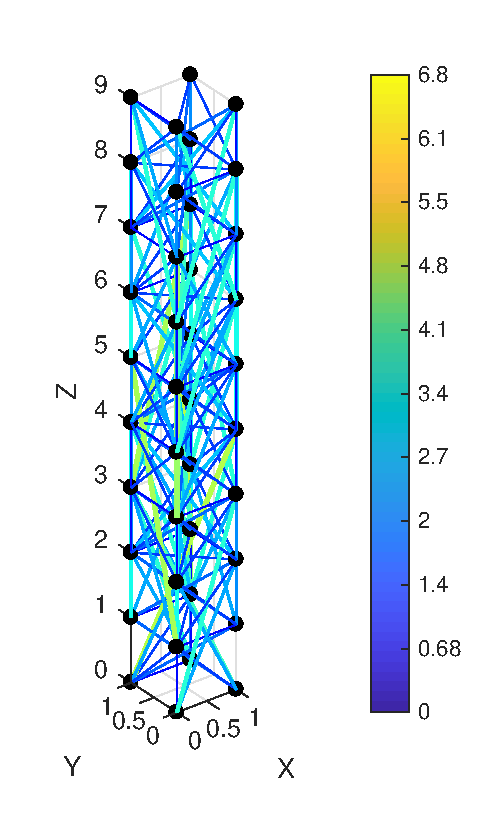
\includegraphics[height=60mm]{fig/column_structure_A}}
 \subfloat[][]{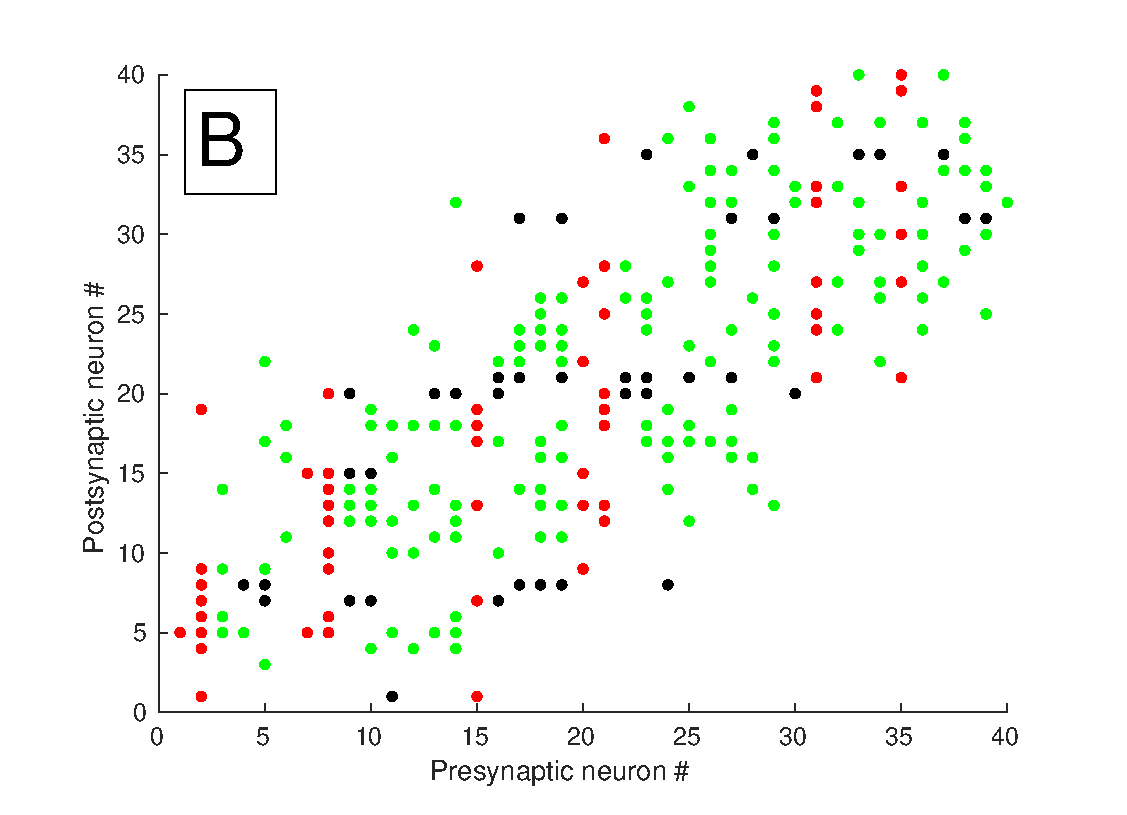
\includegraphics[height=60mm]{fig/column_structure_B}}
 \subfloat[][]{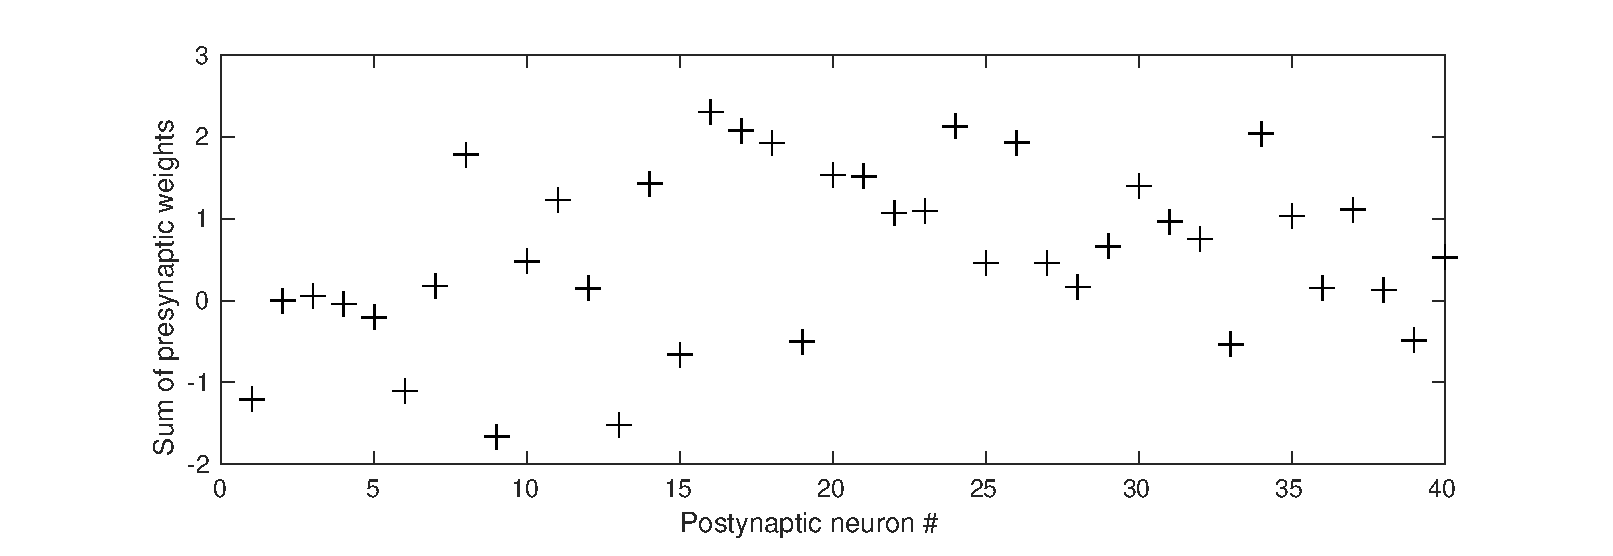
\includegraphics[width=\textwidth]{fig/column_structure_C}}
\end{figure}

A crucial element in neuronal systems is the existence of time delays between the creation of a presynaptic action potential and the arrival of that spike to a target neuron. 
We use distance-dependent time delays for the propagation of a spike from neuron $i$ to neuron $j$ of $\tau_{ij} = \kappa  D(i,j)$. 
The constant of proportionality $\kappa$ ranges from $0$ to $4$.
When $\kappa=0$ the action potential excites the post-synaptic neuron on the succeeding simulation time step.
 
The distribution of post-synaptic connections and delay times are shown in Figure \ref{fig:connection_delay_distrbution} for an example minicolumn.
\begin{figure}[!htb]
 \caption{Distribution of (A) number of post-synaptic connections per neuron and (B) delay time. Data was taken over 100 realizations of a 2x2x50 SCE, $\lambda=2.5$, $\kappa=1$.  } 
 \begin{tabular}{c}
     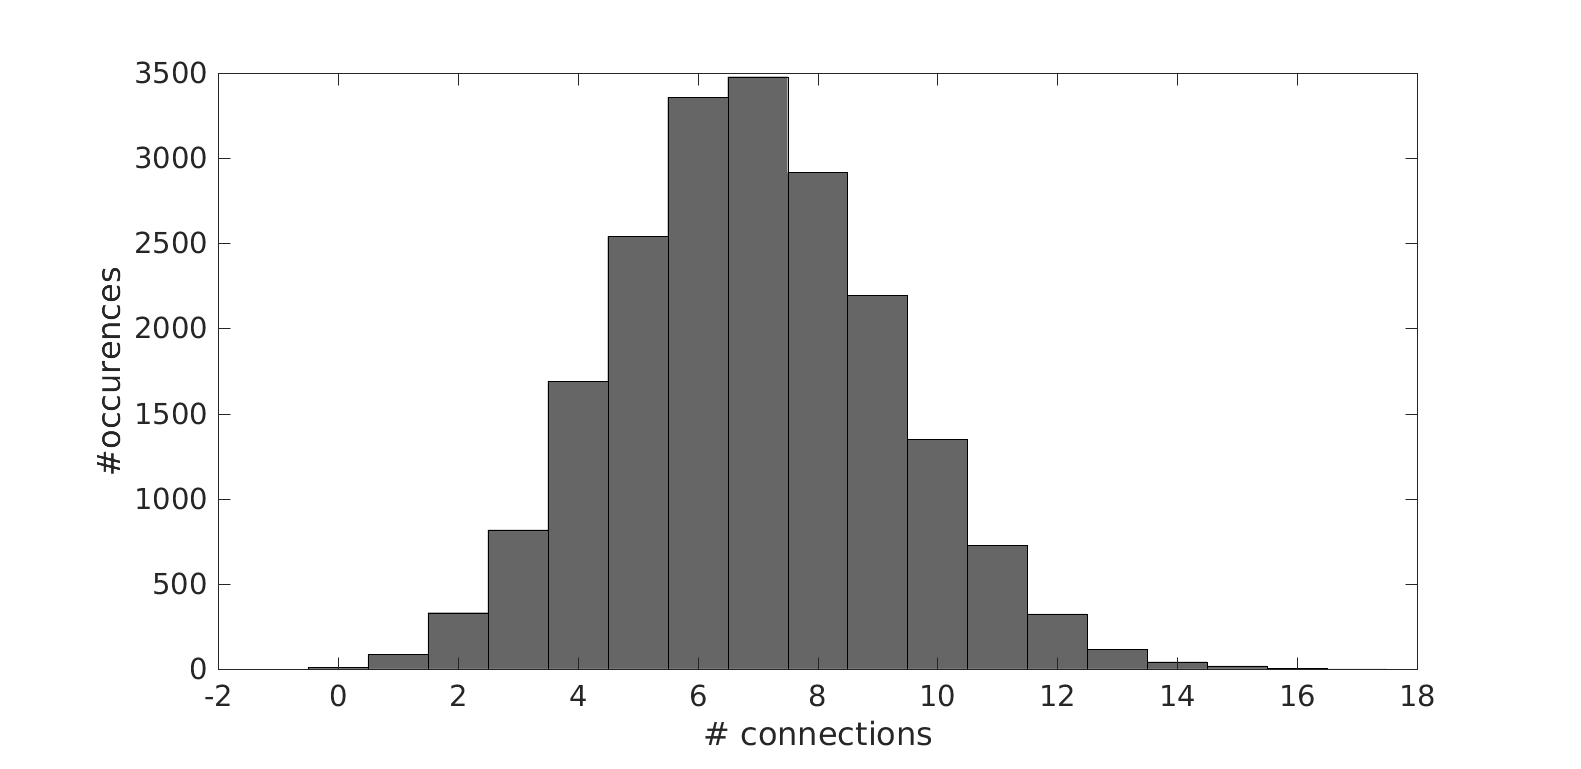
\includegraphics[width=\textwidth]{fig/ConnectionNumberDistribution} \\
     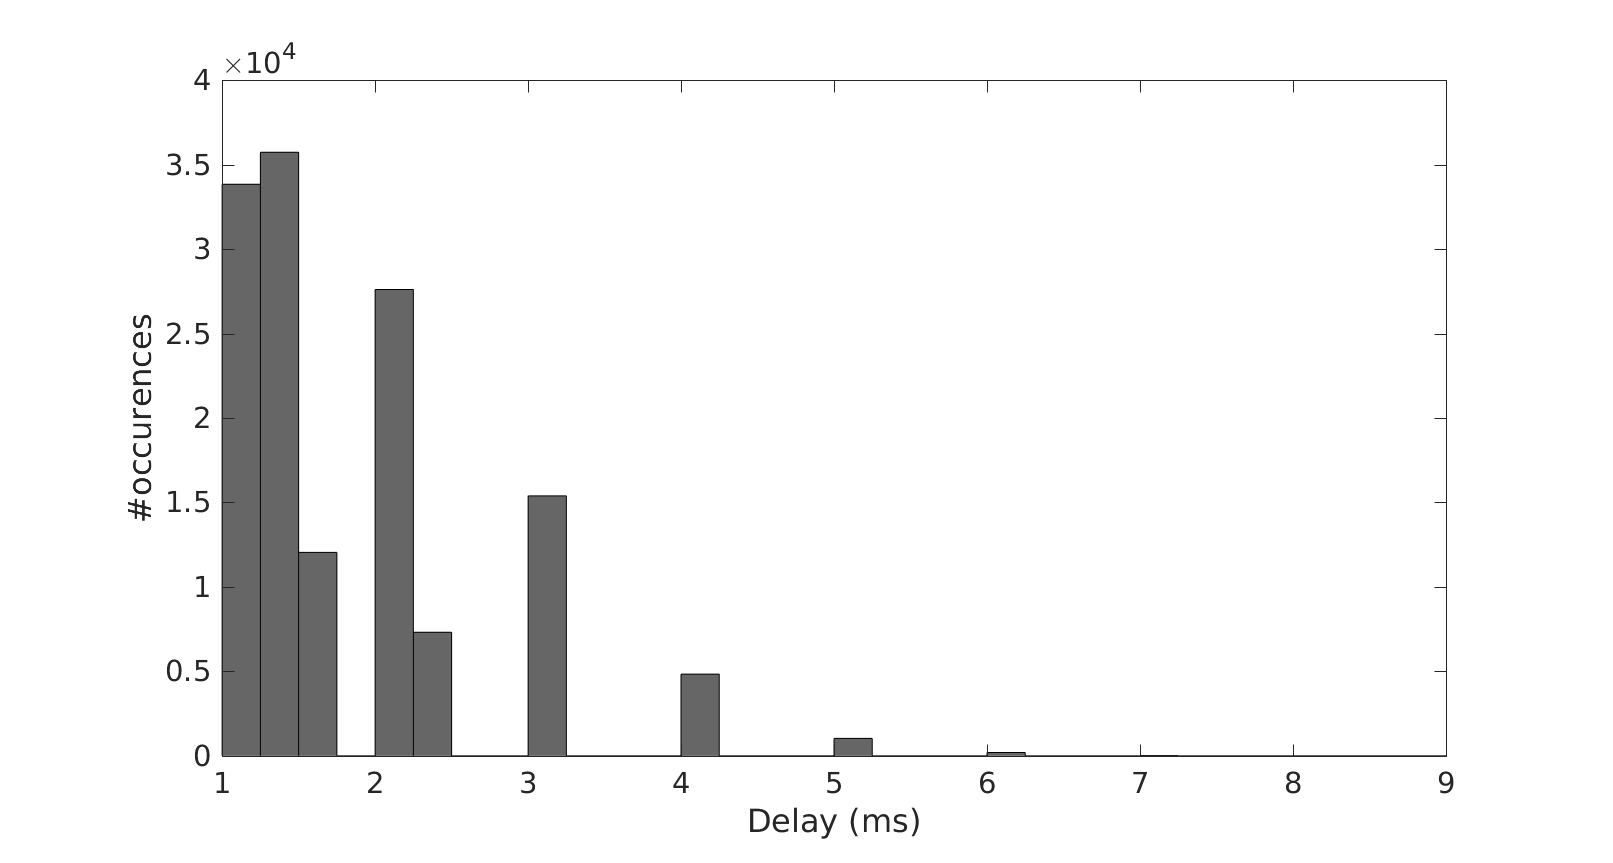
\includegraphics[width=\textwidth]{fig/DelayDistribution} 
 \end{tabular}
 \label{fig:connection_delay_distrbution}
\end{figure}
 \FloatBarrier

We model the firing dynamics of each neuron using the Izhikevich model \citep{izhikevich2003} that consists of a two-dimensional model of two coupled differential equations given by:
\begin{align}
 \begin{split}
  v^\prime &= 0.04v^2+5v+140-u+I \label{eq:neuron_v} \\
  u^\prime &= a(bv-u)
 \end{split}
\end{align}
where $v$ is the membrane potential of the neuron and $u$ is a membrane recovery variable, with a spike threshold and an auxilliary after-spike resetting of parameters by:
\begin{align}
  \text{if } &v>30: v\leftarrow c, u\leftarrow u+d
\end{align}
and I is the sum of all incoming currents to the neuron, explained in detail below. 

Equation \ref{eq:neuron_v} has four parameters (a,b,c,d) that with specific values can model a wide range of neuronal spiking behavior \citep{izhikevich2003}. 
The parameters used here (see Table \ref{tab:izzy_params}) are based on those specified in \citep{izhikevich2003} with modification of the $c$ parameter for excitatory neurons and define a random population of neurons where $U(s,t)$ represent a number drawn from a uniform random distribution between s and t. 
\begin{table}[!htb]
 \caption{Izhikevich model parameters}
 \label{tab:izzy_params}
 \centering
 \begin{tabular}{lcr}
  \textbf{Parameter} & \textbf{Excitatory} & \textbf{Inhibitory} \\
  \hline
  a & 0.02 & 0.02+$\mathcal{U}$(0,0.08) \\
  b & 0.2 & 0.25-$\mathcal{U}(0,0.05)$\\
  c & -65+$\mathcal{U}(0,10)^2$ & -65 \\
  d & 8-$\mathcal{U}(0,6)$& 2 \\
 \end{tabular}
\end{table}
For solving equation (2) numerically we use the modified Euler method from \citep{izhikevich2003} with a time step of $0.2 ms$ except were noted. 


The current I in equation (2) includes the sum of all incoming stimuli into neuron $i$ from other neurons $I_i$ and external stimuli $I_{i,e}$ applied to the system. 
The neuron-neuron incoming current $I_i$ into neuron $i$ is given by:
\begin{align}
 I_i(t) &= \sum_{j\ne i} \sum_{t^\prime_j} S_{ij}  \Theta(t-t^\prime_j-\tau_{ij})e^{-(\frac{t-t^\prime_j-\tau_{ij}}{\sigma_s})^2}
\end{align}

where $t'_j$ are the firing times of neuron $j$, $\Theta$ is the Heaviside step function, and the exponential factor models an exponentially decaying synapse response with a time constant of $\sigma_s = 4 ms$. 
The $S_{ij}$ represent the connection strengths between presynaptic neuron $j$ and postsynaptic neuron $i$ given by
\begin{align}
 \begin{split}
  S_{ij}^{excitatory} &= K \times \mathcal{U}\{0,0.5 \} \\
  S_{ij}^{inhibitory} &= K \times \mathcal{U}\{-1,0 \} 
 \end{split}
\end{align}

where $K$ is a parameter that modulates the strength of connections, with $K=1$ corresponding to the original model in \citep{izhikevich2003}. 

To drive the firing dynamics and create traveling waves we provide stimulation to the systems by using two different and separate external stimulus currents, $I_{i,e}$. 
One of them is a uniform background stimulus applied to each neuron $k$ that depends on whether the neuron is excitatory or inhibitory.
The stimulus values are drawn from a random distribution every $1 ms$ according to:
\begin{align}\label{eq:randomstim}
 \begin{split}
  I_k^{excitatory} &= M \times \mathcal{U}\{0,1 \} \\
  I_k^{inhibitory} &= \frac{2}{5} M \times \mathcal{U}\{0,1 \}
 \end{split}
\end{align}
where $M$ is a parameter that tunes the overall strength of the stimulus, with $M=5$ corresponding to the original model in \citep{izhikevich2003}. 
This stimulus has the effect of creating waves that originate from any point along an SCE and one of the uses is to study interactions between multiple waves in section \ref{sub:wave_initiation}.

The other external stimulus $I_{i,e}$ is a short constant input of current applied to all of the neurons in the lowest ten layers of an SCE. 
The duration of the stimulus is $20 ms$ with a current of strength $5$ units. 
This stimulus has the effect of creating a single wave that can propagate through the total length of an SCE.
One of the uses of this stimulus is to measure the speed of the traveling wave in section \ref{sub:propagation_speed}.

We summarize our model parameters in Table \ref{tab:all_params}. 
\begin{table}[!htb]
 \caption{Model Summary}
 \label{tab:all_params}
 \centering
 \begin{tabular}{c}
  \textbf{Model} \\
  \hline \\
 \end{tabular} \\
 \begin{tabular}{ll}
  Population & Excitatory, inhibitory \\
  Topology & Small columnar ensemble, Z extents $\gg$ X,Y extents \\
  Connectivity & Stochastic, $P_c$ exponentially decays with distance between neurons \\
  Neuron model & Izhikevich model with distribution of neuron parameters \\
  Synapse response & Exponential synaptic response with randomized peak connection strength  \\
  Spike propagation & Delay proportional to distance, Fixed propagation time \\
  Input & Random input to all neurons, Fixed stimulus to neurons at the bottom of the SCE \\
 \end{tabular}
\end{table}

For every simulation we record all of the spikes from all neurons. 
We visualize the spikes in spike raster plots (e.g. Figure \ref{fig:sigma_raster} ).
Because here we focus on traveling waves in the Z direction, we plot the spikes according to the Z position of the neurons.
As a consequence, at each Z position there are multiple neurons that could contribute to the spike raster plot at that Z coordinate (e.g. 4 neurons for the X=2, Y=2 SCE case).

To automatically identify waves we perform a spatial clustering operation to this data to identify spatiotemporal regions identified by high firing density. 
The clustering operation produces an output cluster for any group of more than $3$ spike events that fall within a $20ms$ time window from neurons that are no more than $3$ layers apart.
Each cluster $C(t,z)$ has a time $t$ and position $z$.
This clustering removes random background firing activity. 
The waves are identified using a plane sweep algorithm that proceeds along the dimension of simulation time and applies wave labels to clusters such that all clusters with the same label are part of the same wave.
When a new cluster $C(t,z)$ is encountered, the algorithm associates $C(t,z)$ with any existing wave if the existing wave has a cluster $C(t_c,z_c)$ within $40 ms$ and $6$ units of the new cluster.
If there is no such adjacent cluster a new wave is created using $C(t,z)$ as the first cluster.

An example of the clustering and identification is shown in Figure 2, with further illustration in SI Figure 1.
\begin{figure}[!htb]
 \centering
 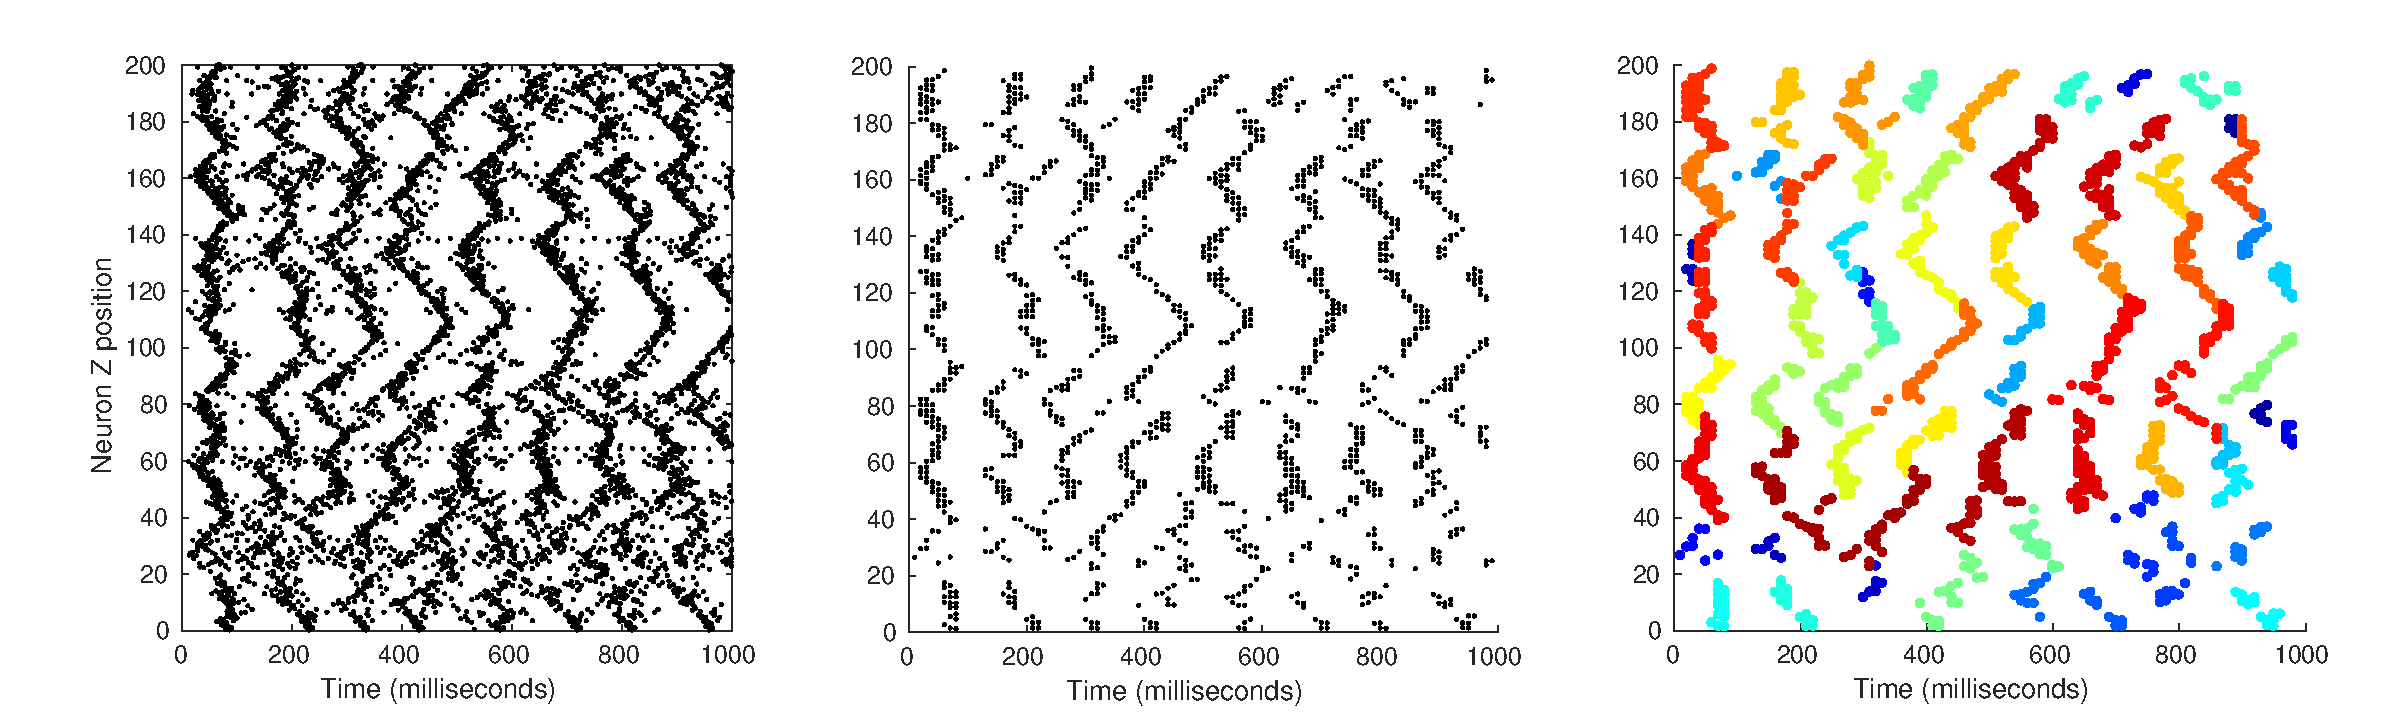
\includegraphics[width=\textwidth]{fig/DetectorExample}
 \caption{Wave identification and labeling using an example SCE with dimensions 2x2x200 . Left: Raster plot of firing events where dots represent neuronal action potentials. 
          Traveling waves can be seen as diagonal structures of dense firing activity. 
          Center: The clustering operation removes background spikes. 
          Right: Individual waves are labeled with unique identifiers color coded in the figure.}
 \label{fig:wave_analysis}
\end{figure}

Our wave detection and analysis approach must remain valid across a range of model parameters. 
We show sample visualizations for varying values of $K$ in Figure \ref{fig:detector_test}.
This detector test demonstrates that our detection and analysis method detects and labels traveling waves of various lengths even in a noisy background.
\begin{figure}[!htb]
 \caption{The clustering and wave labeling process. Spike raster plot (left), filtered clusters (middle) and labeled waves (right, each color is a unique wave) are shown for SCE with different values of $K$. }
 \label{fig:detector_test}
 \centering
   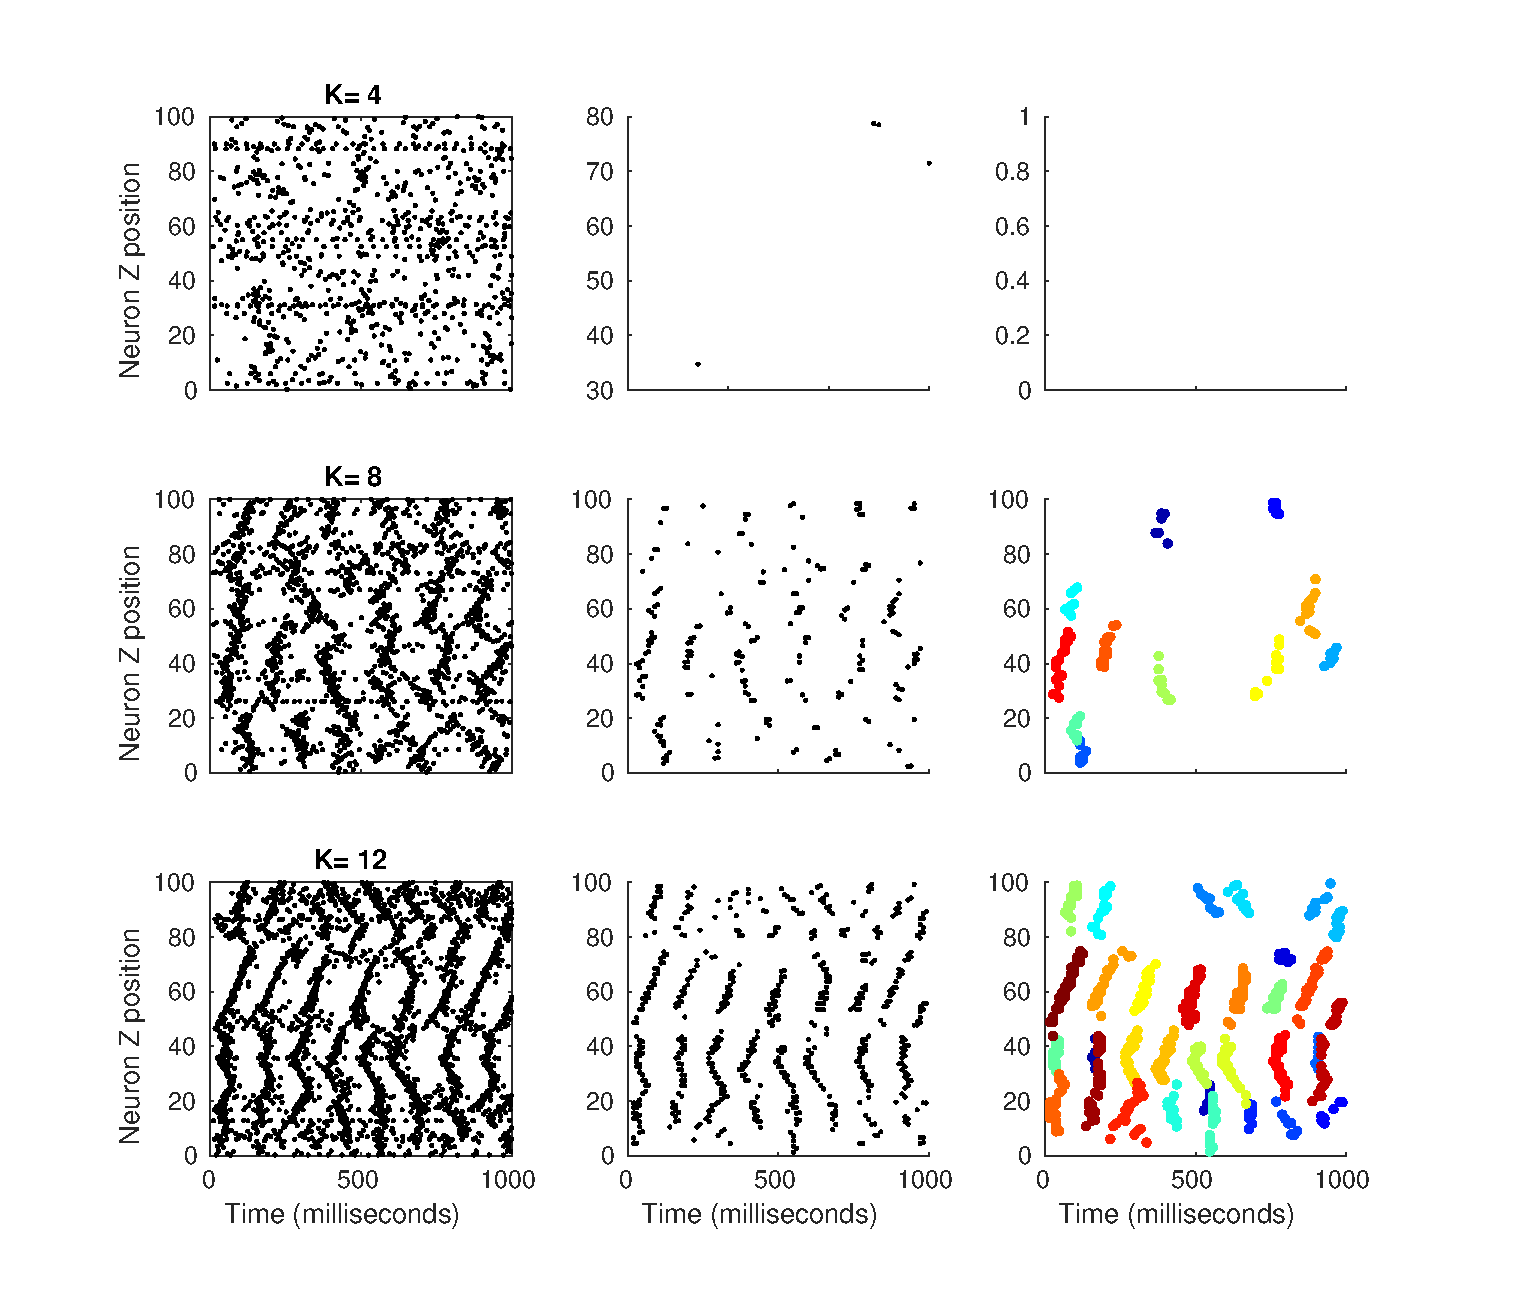
\includegraphics[width=\textwidth]{fig/DetectorTest}
\end{figure}

\FloatBarrier
Once identified and labeled, we measure wave propagation speeds and wave initiation locations. 
We also measure the "wave firing fraction" defined as the fraction of spikes that are associated with the labeled traveling wave (total number of spikes found within the waves divided by number of spikes in the simulation). 

Our exploration of the behavior of traveling waves in an SCE involves testing properties of these waves as a function of the different parameters of our model.
For determining existence of traveling waves we use a $2x2x100$ SCE  with background stimulation (Eq \ref{eq:randomstim}) and vary parameters around a neighborhood of the reference point $\Sigma = \{K=10,\lambda=2.5,P_{exc}=0.8,\kappa=1.0 \}$ that we have determined can sustain traveling waves.
To measure wave propagation speed we use a $2x2x50$ SCE with  a step stimulus applied to the lowest layers of the SCE and adjust our reference point to be $\Sigma_v = \{K=24,\lambda=2.5,P_{exc}=0.8,\kappa=1.0 \}$.
This reference point was selected after inspecting the SCE behavior under a wide range of parameter values.
The increase in $K$ is required when using the step stimulus because the higher layers of the SCE do not receive any stimulus.
This requires stronger connections so that the traveling wave can elicit spikes from neurons resting at equilibrium.

\FloatBarrier

\endinput
%%
%% End of file `example-1.tex'.
